\chapter{Experiments}\label{sec:experiments}

In this section, the performed experiments are presented, and results of the
experiments are shown. The two experiments were performed on the workstation
described in Section \ref{sec:setup}. Both experiments were programmed in
Python, and open-source software projects for the models and environment were
used extensively.

\section{Characterizing Meta Reinforcement Learning}

The objective of the first experiment was to evaluate the adaptiveness and
reduce in retraining time with meta \rl. The evaluation is done using the meta
\rl offloading model, called \mrlco, proposed in \citeA{wang2020}. The data
was converted into \DAG data (see \ref{sec:data}). Running the experiments
with the converted data required modifications in the source code of \mrlco.
The modifications were made in the \code{meta\_trainer.py} file. There was a
list of directories containing 100 graph data files, which was changed into the
directories with the Euro-Argo data. More modifications have been done to fix
bugs, e.g. adding in logic for taking the maximum value of an array when it is
empty.

After the bug fixing, running the model was possible. Each run consisted of
2,000 iterations in batch sizes of 100. After each batch a TensorFlow
checkpoint was saved on disk. Every iteration it appended a row of data to a
comma separated value (csv) file. The following aspects of each iteration were
saved:

\begin{itemize}[noitemsep]
    \item Iteration
    \item Number of trajectories
    \item Average reward
    \item Execution time:
        \begin{itemize}[noitemsep]
            \item Policy execution time
            \item Environment execution time
        \end{itemize}
    \item Return value:
        \begin{itemize}[noitemsep]
            \item Average return value
            \item Minimal return value
            \item Maximal return value
            \item Standard deviation of return value
            \item Average discounted return
        \end{itemize}
    \item Latency:
        \begin{itemize}[noitemsep]
            \item Average latency
            \item Average greedy latency
        \end{itemize}
\end{itemize}

\begin{figure}[htp!]
    \centering
    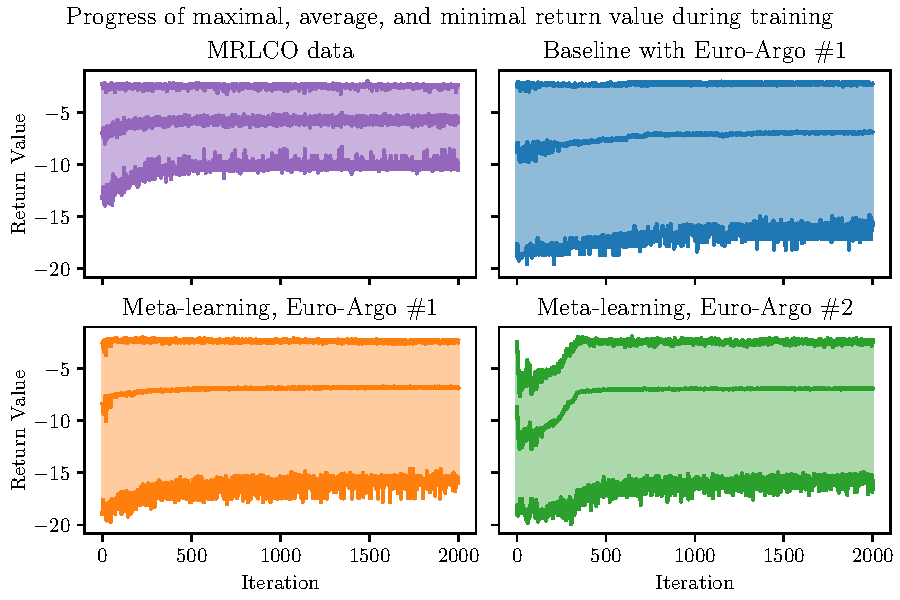
\includegraphics[width=\textwidth]{./fig/return.pdf}
    \caption{The progress of the return value during training. The upper line
    plots the maximal return value per iteration, the middle line the average
    return value and the lower line plots the minimal return value per
    iteration. The \#1 and \#2 are respectively the first and second batch of
    the Euro-Argo data.}
    \label{fig:return}
\end{figure}


\begin{table}[htp!]
    \centering
    \caption{The average policy and environment execution time per run. The
    values are in seconds.}
    \label{table:exectime}
    \begin{tabular}{l|lccc}
        ID & Batch & Policy & Environment & Total\\ \hline
        1  & 1     & 4955   & 1907 & 6862\\
        2  & 1     & 4971   & 1907 & 6878\\
        3  & 2     & 5013   & 1822 & 6835
    \end{tabular}
\end{table}


\subsection{Recreating MRLCO Results}

The first experiment was recreating the results from the paper. This was done
by running the \mrlco model without changes on the provided data. The two runs
are plotted in Figure \large{TODO}\normalsize. It is visible that the second run
converges quicker due to meta-learning. The reward in the last iteration of
training was $-5.42$. The average return value at the last iteration was
$-5.60$.


\subsection{MRLCO with Euro-Argo Data}

\begin{figure}[htp!]
    \centering
    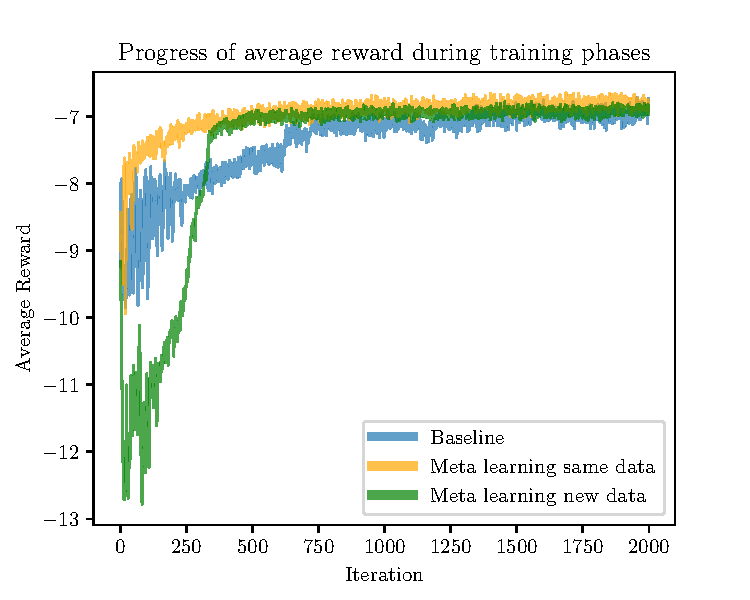
\includegraphics[width=.7\textwidth]{./fig/reward.pdf}
    \caption{The progress of average reward during training on \mrlco and
    Euro-Argo log data. The average reward on the \mrlco data seems to variate much
    more than on our data. The \mrlco data delivers a higher reward.}
    \label{fig:rewards}
\end{figure}


The second set of experiments was done with the converted Euro-Argo data.
Three training phases were done. The first training phase was a baseline run,
without any meta-learning up front. It was trained on the first half of the
data: 1500 graph files. This half will from now on be called batch 1, the
other half batch 2. After 1955 iterations the baseline model reached its
optimal reward of -6.7. Now the baseline model is trained, it can be used for
meta-learning. Two meta-learning runs were done: one with the exact same data,
batch 1 and another one with different data from the same distribution, batch
2. These runs reached their optimal reward after respectively 521 and 920
iterations. The real time of these iterations are listed in
\ref{table:max-reward}. In the table it is shown that the training time
speedup on the same data is 105 minutes, from almost three hours to a bit more
than one hour. The training time speedup on new data is 54 minutes. The time
difference between the full training sessions is not significant. In Table
\ref{table:exectime}, the total execution times for policy and environment are
shown. The difference in execution time between the different runs are only a
couple seconds. The maximal reward on the second data batch is -6.8, a 0.1
difference with the maximal reward from the base line model. The progress of
average reward for all three training phases are plotted in Figure
\ref{fig:rewards}. In this figure it is clear that the meta-learned runs
achieve their optimal policy in an earlier iteration. Even when the reward at
the start is much lower, it still learns very quick using meta-learning.

The return value is plotted in Figure \ref{fig:return}. The difference in return
values between the runs using Euro-Argo is not significant. There is however a
difference with the \mrlco data, which has a higher minimal return value. No
reason is found for this difference. The maximal and average return value are
around the same value.

\begin{table}[htp!]
    \centering
    \caption{The time it takes to converge to the maximal average reward
    (-6.8). The time is expressed as the number of iterations and the real
    (sometimes called wallclock) time. An experiment of 2000 iterations took
    255 minutes and 10 seconds (15310 seconds). The time to converge thus is
    calculated using the following formula: $\protect it / 2000 \cdot 15310$.}
    \label{table:max-reward}
    \begin{tabular}{c|lrr}
        ID & Batch & Iterations & Time (min)\\ \hline
        1 & 1 & 1345 & 171\\
        2 & 1 & 521 & 66\\
        3 & 2 & 920 & 117\\
    \end{tabular}
\end{table}



\section{Comparing Reinforcement Learning Model in OpenAI Gym}

The second group of experiments were done to evaluate multiple \rl algorithms
as schedulers. A side objective of this experiment was to have a good testbed
for other experiments in this research project. OpenAI's Gym was chosen for
this because of its popularity and simplicity. As described in Section
\ref{sec:evaluation} and Section \ref{sec:setup} OpenAI is a popular platform
for creating, testing and evaluating reinforcement learning models. The
environment used in this experiment is described in Section
\ref{sec:taillard}. The \jss environment (\code{JSSEnv}) in combination with
the \code{keras-rl} package\footlink{github.com/keras-rl/keras-rl}, would allow
to experiment with many different \rl algorithms and evaluate their
performance as scheduler. The \code{keras-rl} package currently supports
\acrfull{dqn} \cite{mnih2013}, Double \dqn \cite{hasselt2016}, Deep
Deterministic Policy Gradient \cite{lillicrap2015}, Continuous \dqn
\cite{gu2016}, Cross-Entropy Method \cite{szita2006}, Dueling network \dqn
(Dueling \dqn) \cite{wang2016}, and Deep SARSA. Simulating the agent in the
\jss environment required very little code. As start make the Gym environment,
after this define a \nn (shown in Figure \ref{fig:neuralnetwork}),
then define a \rl agent providing a policy and the \nn and at last fit the
agent on the environment.

\begin{figure}[htp!]
    \centering
    
\includegraphics[width=\textwidth]{./fig/nn.png}
    \caption{The \dnns used in the \rl models from \code{keras-rl}.}
    \label{fig:neuralnetwork}
\end{figure}


Starting the experiment, a FIFO scheduler in the environment was run. The
makespan after this run was 5724 and the final reward was -5.80, and the
average reward was 0.40. After this general Q-learning and the deep \rl
algorithms mentioned above were tried. There were no results due to various
errors, which will be discussed in detail in Section \ref{sec:discussion}.
